\let\negmedspace\undefined
\let\negthickspace\undefined
\documentclass[journal]{IEEEtran}
\usepackage[a5paper, margin=10mm, onecolumn]{geometry}
\usepackage{lmodern} 
\usepackage{tfrupee} 

\setlength{\headheight}{1cm} 
\setlength{\headsep}{0mm}     

\usepackage{gvv-book}
\usepackage{gvv}
\usepackage{cite}
\usepackage{amsmath,amssymb,amsfonts,amsthm}
\usepackage{algorithmic}
\usepackage{graphicx}
\usepackage{textcomp}
\usepackage{xcolor}
\usepackage{txfonts}
\usepackage{listings}
\usepackage{enumitem}
\usepackage{mathtools}
\usepackage{gensymb}
\usepackage{comment}
\usepackage{multicol}
\usepackage[breaklinks=true]{hyperref}
\usepackage{tkz-euclide} 
\usepackage{listing}

\graphicspath{ {./figs/} }

\begin{document}


\title{
ASSIGNMENT 1: GATE 2007 \\
IN:INSTRUMENTATION ENGINEERING}
\author{AI25BTECH11013-Gautham Pocha}
\maketitle
\renewcommand{\thefigure}{\theenumi}
\renewcommand{\thetable}{\theenumi}
\begin{enumerate}

 \item Let $A$ be an $n \times n$ real matrix such that $A^2 = I$ and $y$ be an $n$--dimensional vector. Then the linear system of equations $Ax = y$ has  
\begin{enumerate}
\item no solution
\item a unique solution
\item more than one but finitely many independent solutions
\item infinitely many independent solutions
\end{enumerate}
\hfill(GATE IN 2007)
\item Let $j = \sqrt{-1}$. Then one value of $j^j$ is  
\begin{multicols}{4}
\begin{enumerate}
\item $\sqrt{j}$
\item $-1$
\item $\pi/2$
\item $e^{-\pi/2}$
\end{enumerate}
\end{multicols}
\hfill(GATE IN 2007)
\item In full sunlight, a solar cell has a short circuit current of $75$ mA and a current of $70$ mA for a terminal voltage of $0.6$ V with a given load. The Thevenin resistance of the solar cell is  
\begin{multicols}{4}
\begin{enumerate}
\item $8~\Omega$
\item $8.6~\Omega$
\item $120~\Omega$
\item $240~\Omega$
\end{enumerate}
\end{multicols}
\hfill(GATE IN 2007)
 \item The DC voltage gain $\frac{V_o}{V_i}$ in the following circuit is given by  
\begin{figure}[H]
    \centering
      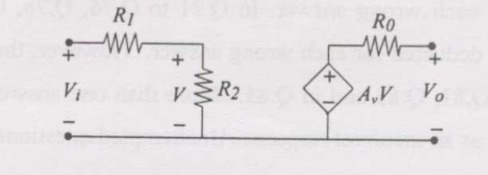
\includegraphics[width=0.6\textwidth]{1.jpg} 
      \caption{}
    \label{fig:fig1} 
\end{figure}
\begin{multicols}{2}
\begin{enumerate}
\item $A_v \frac{R_2}{R_1 + R_2}$
\item $A_v \frac{R_1}{R_1 + R_2}$
\item $A_v \frac{R_2}{R_1 + R_2 + R_0}$
\item $A_v$
\end{enumerate}
\end{multicols}
\hfill(GATE IN 2007)

\item Match the essential amplifier characteristics with the sensing applications given below: \\
\begin{table}[H]
\centering
\begin{tabular}{p{4cm} p{4cm}}
\textbf{Amplifier Characteristics} & \textbf{Sensing Applications} \\
\hline
P. Charge amplifier with very low bias current and high input impedance & L. Strain gauge in unipolar DC Wheatstone bridge \\
Q. Voltage amplifier with low bias current and very high input impedance & M. Glass electrode pH sensor \\
R. Voltage amplifier with very high CMRR & N. Piezoelectric sensor for measurement of static force \\
\end{tabular}
\caption{}
\label{tab:matching 1}
\end{table}
\begin{multicols}{2}
\begin{enumerate}
\item P-L, Q-M, R-N
\item P-M, Q-N, R-L
\item P-N, Q-L, R-M
\item P-N, Q-M, R-L
\end{enumerate}
\end{multicols}
\hfill(GATE IN 2007)
\item The figure below shows various configurations of bonding a strain gauge to a cantilever subjected to a bending force $F$.  
\begin{figure}[H]
    \centering
      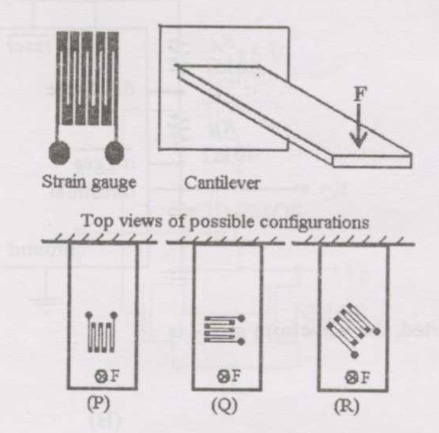
\includegraphics[width=0.6\textwidth]{2.jpg} 
      \caption{}
    \label{fig:fig2} 
\end{figure}
Which configuration gives the maximum change in resistance for this force?
\begin{enumerate}
\item P  
\item Q  
\item R  
\item All have equal change in resistance
\end{enumerate}
\hfill(GATE IN 2007)
\item When light falls on the photodiode shown in the following circuit, the reverse saturation current of the photodiode changes from 100 $\mu$A to 200 $\mu$A.  
\begin{figure}[H]
    \centering
      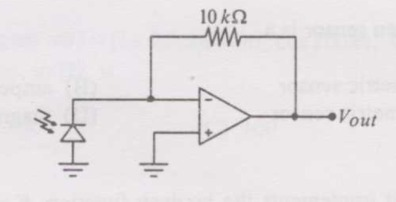
\includegraphics[width=0.6\textwidth]{3.jpg} 
      \caption{}
    \label{fig:fig3} 
\end{figure}
Assuming the op-amp to be ideal, the output voltage $V_{out}$ of the circuit
\begin{enumerate}
\item does not change  
\item changes from 1 V to 2 V  
\item changes from 2 V to 1 V  
\item changes from -1 V to -2 V
\end{enumerate}
\hfill(GATE IN 2007)

\item A 555 astable multivibrator circuit is shown.  
\begin{figure}[H]
    \centering
      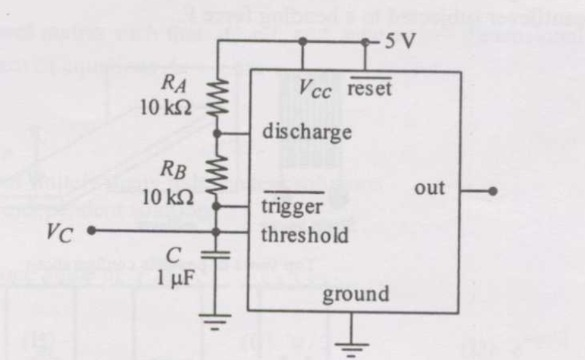
\includegraphics[width=0.6\textwidth]{4.jpg} 
      \caption{}
    \label{fig:fig4} 
\end{figure}
If $R_B$ is shorted,\hfill(GATE IN 2007) the waveform at $V_C$ is
\begin{multicols}{2}
\begin{enumerate}
\item \begin{figure}[H]
      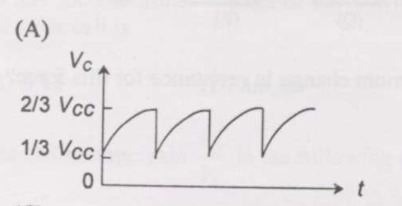
\includegraphics[width=0.3\textwidth]{5.jpg} 
      \caption{}
    \label{fig:fig5} 
    \end{figure}  
\item   \begin{figure}[H]
      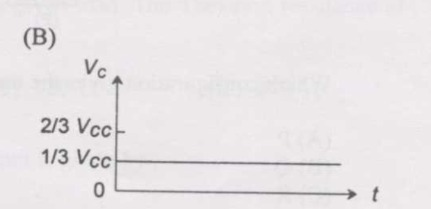
\includegraphics[width=0.3\textwidth]{6.jpg} 
      \caption{}
    \label{fig:fig6} 
\end{figure}
\item \begin{figure}[H]
      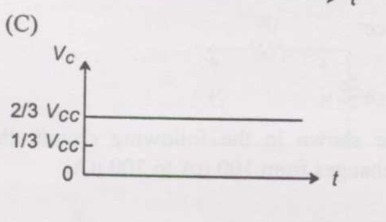
\includegraphics[width=0.3\textwidth]{7.jpg} 
      \caption{}
    \label{fig:fig7} 
\end{figure}
\item  \begin{figure}[H]
      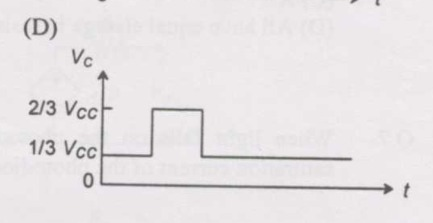
\includegraphics[width=0.3\textwidth]{8.jpg} 
      \caption{}
    \label{fig:fig8} 
\end{figure} 
\end{enumerate}
\end{multicols}
\hfill(GATE IN 2007)
\item A Clark oxygen sensor is a
\begin{multicols}{2}
\begin{enumerate}
\item potentiometric sensor  
\item amperometric sensor  
\item conductometric sensor  
\item magnetostrictive sensor  
\end{enumerate}
\end{multicols}
\hfill(GATE IN 2007)
\item A logic circuit implements the Boolean function$F = \overline{X} \cdot Y + X \cdot \overline{Y} \cdot \overline{Z}$It is found that the input combination $ X = Y = 1 $ can never occur. Taking this into account, a simplified expression for $ F $ is:
\begin{multicols}{2}
\begin{enumerate}
\item $ \overline{X} + \overline{Y} \cdot \overline{Z} $
\item $ X + Z $
\item $ X + Y $
\item $ Y + X \cdot \overline{Z} $
\end{enumerate}
\end{multicols}
\hfill(GATE IN 2007)
\item A CMOS implementation of a logic gate is shown in the following figure.
\begin{figure}[H]
    \centering
      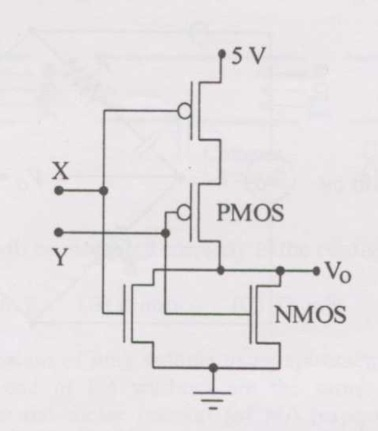
\includegraphics[width=0.6\textwidth]{9.jpg} 
      \caption{}
    \label{fig:fig9} 
\end{figure}
The boolean logic function realized by the circuit is
\begin{multicols}{4}
\begin{enumerate}
\item AND  
\item NAND  
\item NOR  
\item OR  
\end{enumerate}
\end{multicols}
\hfill(GATE IN 2007)

\item Let $x(t)$ be a continuous-time, real-valued signal band-limited to $F$ Hz.  
The Nyquist sampling rate, in Hz, for $y(t) = x(0.5t) + x(t) - x(2t)$ is
\begin{multicols}{4}
\begin{enumerate}
\item $F$  
\item $2F$  
\item $4F$  
\item $8F$  
\end{enumerate}
\end{multicols}
\hfill(GATE IN 2007)
\item Consider the periodic signal $x(t) = (1 + 0.5\cos 40\pi t)\cos 200\pi t$, where $t$ is in seconds.  
Its fundamental frequency, in Hz, is
\begin{multicols}{4}
\begin{enumerate}
\item 20  
\item 40  
\item 100  
\item 200  
\end{enumerate}
\end{multicols}
\hfill(GATE IN 2007)
\item A dynamometer type wattmeter with a single scale marked for the smallest power range, has two current ranges, namely, 0--5 A and 0--10 A as well as two voltage ranges, namely, 0--150 V and 0--300 V.  
To carry out a load test on a 230 V / 115 V, 1 kVA, single phase transformer, the wattmeter is used on the high voltage side.  
The voltage and current ranges are chosen for maximum utilization of the scale. The multiplying factor to be used in this case is
\begin{multicols}{4}
\begin{enumerate}
\item 0.5  
\item 1.0  
\item 2.0  
\item 4.0  
\end{enumerate}
\end{multicols}
\hfill(GATE IN 2007)
\item Consider the AC bridge shown, with $A, L$ and $C$ having positive finite values. 
\begin{figure}[H]
    \centering
      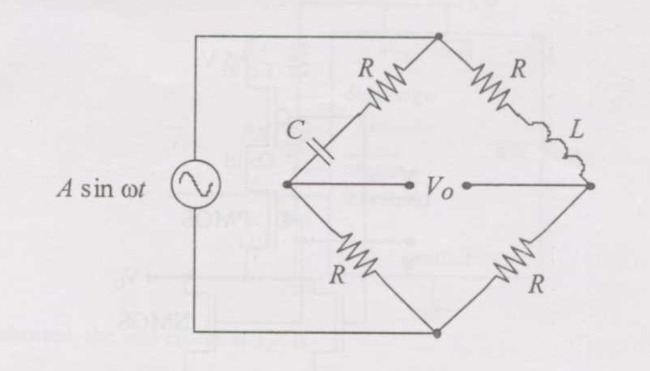
\includegraphics[width=0.6\textwidth]{10.jpg} 
      \caption{}
    \label{fig:fig10} 
\end{figure}
Then
\begin{multicols}{2}
\begin{enumerate}
\item $V_o = 0$ if $\omega L = \dfrac{1}{\omega C}$  
\item $V_o = 0$ if $L = C$  
\item $V_o = 0$ if $R = \dfrac{1}{\omega \sqrt{LC}}$  
\item $V_o$ cannot be made zero  
\end{enumerate}
\end{multicols}
\hfill(GATE IN 2007)
\item A feedback control system with high gain $K$, is shown. 
\begin{figure}[H]
    \centering
      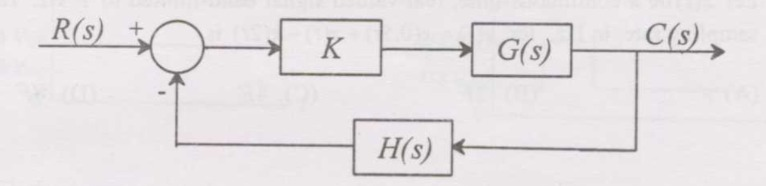
\includegraphics[width=0.6\textwidth]{11.jpg} 
      \caption{}
    \label{fig:fig11} 
\end{figure}
Then the closed loop transfer function is
\begin{enumerate}
\item sensitive to perturbations in $G(s)$ and $H(s)$  
\item sensitive to perturbations in $G(s)$ but not to perturbations in $H(s)$  
\item sensitive to perturbations in $H(s)$ but not to perturbations in $G(s)$  
\item insensitive to perturbations in $G(s)$ and $H(s)$  
\end{enumerate}
\hfill(GATE IN 2007)
\item Consider the following standard state-space description of a linear time-invariant single input single output system:  
$\dot{x} = Ax + Bu, \quad y = Cx + Du$  

Which one of the following statements about the transfer function \textbf{CANNOT} be true if $D \neq 0$?
\begin{multicols}{2}
\begin{enumerate}
\item The system is unstable  
\item The system is strictly proper  
\item The system is low pass  
\item The system is of type zero  
\end{enumerate}
\end{multicols}
\hfill(GATE IN 2007)

\item During intravascular measurement of arterial blood pressure, catheters may be introduced in different configurations, as shown in the figures below.  
\begin{figure}[H]
    \centering
      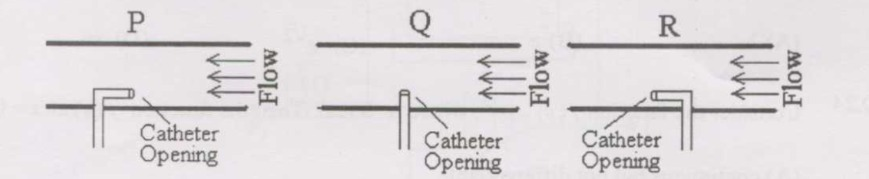
\includegraphics[width=0.6\textwidth]{12.jpg} 
      \caption{}
    \label{fig:fig12} 
\end{figure}
The static pressure will be measured correctly in the configuration(s)
\begin{multicols}{2}
\begin{enumerate}
\item P and Q but not in R  
\item R only  
\item Q only  
\item P and R but not in Q  
\end{enumerate}
\end{multicols}
\hfill(GATE IN 2007)
\item In $ \text{N}_2 $-washout estimation of lung volume using spirometry, the lung volumes at the beginning and the end of the washout are the same. Let $ T, V, F $ denote temperature, volume and molar fraction (of $ \text{N}_2 $) respectively; subscripts $ S $ and $ L $ denote the spirometer and the lung; and $ t_1, t_2 $ the beginning and end times of the experiment, respectively. Then:
\begin{multicols}{2}
\begin{enumerate}
\item $ V_L = \dfrac{T_L}{T_S} \left[ \dfrac{F_S(t_2)V_S(t_2)}{F_L(t_1) - F_L(t_2)} \right] $
\item $ V_L = \dfrac{T_L}{T_S} \left[ \dfrac{F_L(t_2)V_S(t_2)}{F_L(t_1) - F_L(t_2)} \right] $
\item $ V_L = F_L(t_1)V_L(t_2) $
\item $ V_L = T_S F_S(t_2)V_S(t_2) $
\end{enumerate}
\end{multicols}
\hfill(GATE IN 2007)

\item The dispersion in an X-ray diffractometer, defined as $\dfrac{d\theta}{d\lambda}$, is given by the expression  
\begin{multicols}{4}
\begin{enumerate}
\item $\dfrac{m}{2d \cos \theta}$  
\item $\dfrac{m}{2d \sin \theta}$  
\item $2d \sin \theta$  
\item $2d \cos \theta$  
\end{enumerate}
\end{multicols}
\hfill(GATE IN 2007)

\item The polynomial $p(x) = x^5 + x^2 + 2$ has  
\begin{multicols}{2}
\begin{enumerate}
\item all real roots  
\item 3 real and 2 complex roots  
\item 1 real and 4 complex roots  
\item all complex roots  
\end{enumerate}
\end{multicols}

\hfill(GATE IN 2007)
\item Let $A = [a_{ij}], 1 \leq i,j \leq n,$ with $n \geq 3$ and $a_{ij} = i+j$. Then the rank of $A$ is  
	\begin{multicols}{4}
\begin{enumerate}
\item 0  
\item 1  
\item $n-1$  
\item n  
\end{enumerate}
\end{multicols}
\hfill(GATE IN 2007)

\item For real $ x $, the maximum value of $ \dfrac{e^{\sin x}}{e^{\cos x}} $ is:
\begin{multicols}{2}
\begin{enumerate}
\item 1
\item $ e $
\item $ e^{\sqrt{2}} $
\item $ \infty $
\end{enumerate}
\end{multicols}
\hfill(GATE IN 2007)

\item Consider the function $f(x) = |x|^3$, where $x$ is real. Then the function $f(x)$ at $x=0$ is 
\begin{enumerate}
\item continuous but not differentiable  
\item once differentiable but not twice  
\item twice differentiable but not thrice  
\item thrice differentiable  
\end{enumerate}
\hfill(GATE IN 2007)

\item The value of the integral $\int_{0}^{\infty} \int_{0}^{\infty} e^{-x^2-y^2} \, dx\, dy$ is  
\begin{multicols}{4}
\begin{enumerate}
\item $\sqrt{\pi}/2$  
\item $\sqrt{\pi}$  
\item $\pi$  
\item $\pi/4$  
\end{enumerate}
\end{multicols}
\hfill(GATE IN 2007)

\item For the function $\dfrac{\sin z}{z^3}$ of a complex variable, the point $z=0$ is  
\begin{multicols}{2}
\begin{enumerate}
\item a pole of order 3  
\item a pole of order 2  
\item a pole of order 1  
\item not a singularity  
\end{enumerate}
\end{multicols}
\hfill(GATE IN 2007)

\item Assume that the duration in minutes of a telephone conversation follows the exponential distribution $f(x) = \dfrac{1}{5} e^{-x/5}, x \geq 0$. The probability that the conversation will exceed five minutes is  
\begin{multicols}{4}
\begin{enumerate}
\item $\dfrac{1}{e}$  
\item $\dfrac{1}{5}$  
\item $\dfrac{1}{3}$  
\item $1 - \dfrac{1}{e}$  
\end{enumerate}
\end{multicols}
\hfill(GATE IN 2007)

\item The boundary-value problem $y'' + \lambda y = 0, \, y(0)=y(\pi)=0$ will have non-zero solutions if and only if the values of $\lambda$ are  
\begin{multicols}{2}
\begin{enumerate}
\item 0, $\pm 1, \pm 2, \dots$  
\item 1, 2, 3, \dots  
\item 1, 4, 9, \dots  
\item 1, 9, 25, \dots  
\end{enumerate}
\end{multicols}

\hfill(GATE IN 2007)
\item Identify the Newton-Raphson iteration scheme for finding the square root of 2.  
\begin{multicols}{2}
\begin{enumerate}
\item $x_{n+1} = \dfrac{1}{2} \left(x_n + \dfrac{2}{x_n}\right)$  
\item $x_{n+1} = \dfrac{1}{2} \left(x_n - \dfrac{2}{x_n}\right)$  
\item $x_{n+1} = \dfrac{2}{x_n}$  
\item $x_{n+1} = \sqrt{2}\,x_n$  
\end{enumerate}
\end{multicols}
\hfill(GATE IN 2007)

\item Consider the linear circuit with an ideal op-amp shown in the figure below.  
\begin{figure}[H]
    \centering
      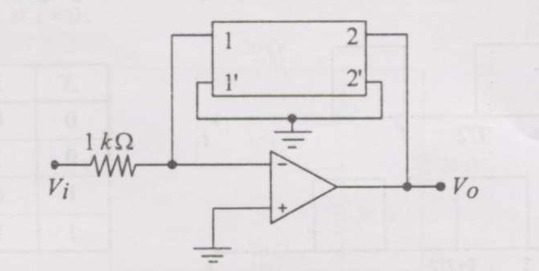
\includegraphics[width=0.6\textwidth]{13.jpg} 
      \caption{}
    \label{fig:fig13} 
\end{figure}
The $Z$-parameters of the two-port feedback network are $Z_{11} = Z_{22} = 11 \, k\Omega$ and $Z_{12} = Z_{21} = 1 \, k\Omega$. The gain of the amplifier is  
\begin{multicols}{4}
\begin{enumerate}
\item +110  
\item +11  
\item -1  
\item -120  
\end{enumerate}
\end{multicols}
\hfill(GATE IN 2007)

\item Consider a non-ideal voltage source whose output voltage is measured by a non-ideal voltmeter as shown below. 
\begin{figure}[H]
    \centering
      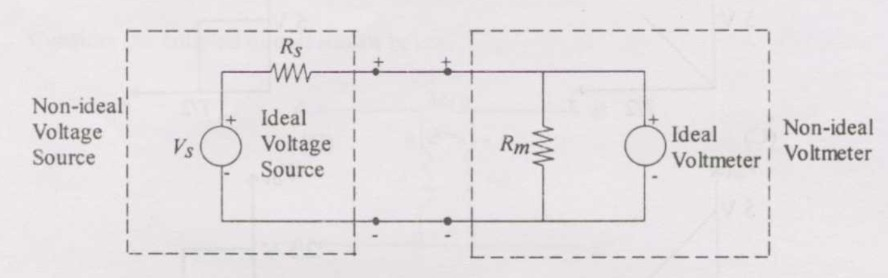
\includegraphics[width=0.6\textwidth]{14.jpg} 
      \caption{}
    \label{fig:fig14} 
\end{figure}
Let $V_d$ be the difference between $V_s$ and the measured voltage. Then $V_d$ is a function of  
\begin{multicols}{2}
\begin{enumerate}
\item $R_s$ only  
\item $R_m$ only  
\item $\dfrac{R_s}{R_m}$  
\item $R_s - R_m$  
\end{enumerate}
\end{multicols}
\hfill(GATE IN 2007)

\item Two sensors have measurement errors that are Gaussian distributed with zero means and variances $\sigma_1^2$ and $\sigma_2^2$, respectively. The two sensor measurements $x_1$ and $x_2$ are combined to form the weighted average $x = \alpha x_1 + (1-\alpha)x_2, \, 0 \leq \alpha \leq 1$. Assuming that the measurement errors of the two sensors are uncorrelated, the weighting factor $\alpha$ that yields the smallest error variance of $x$ is  
\begin{multicols}{4}
\begin{enumerate}
\item $\dfrac{\sigma_1^2}{\sigma_1^2 + \sigma_2^2}$  
\item $\dfrac{\sigma_2^2}{\sigma_1^2 + \sigma_2^2}$  
\item $\dfrac{\sigma_1}{\sigma_1 + \sigma_2}$  
\item 0.5  
\end{enumerate}
\end{multicols}
\hfill(GATE IN 2007)
\item Two square waves of equal period $T$, but with a time delay $\tau$ are applied to a digital circuit whose truth table is shown in the following figure.  
\begin{figure}[H]
    \centering
      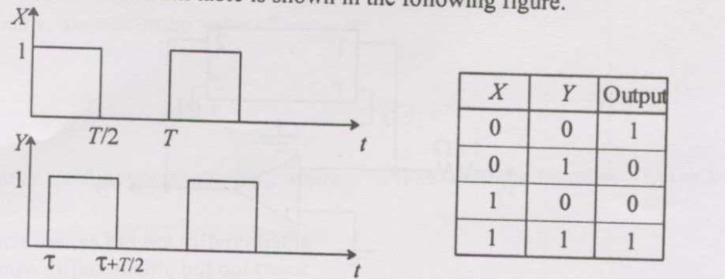
\includegraphics[width=0.6\textwidth]{15.jpg} 
      \caption{}
    \label{fig:fig15} 
\end{figure}
The high and low levels of the output of the digital circuit are $5\ \mathrm{V}$ and $0\ \mathrm{V}$, respectively. Which one of the following figures shows the correct variation that the output voltage is a function of $\tau$ for $0 \leq \tau \leq T/2$?

\begin{enumerate}
\item \begin{figure}[H]
      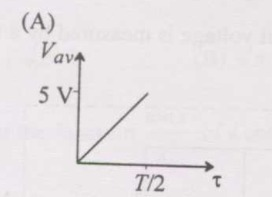
\includegraphics[width=0.3\textwidth]{16.jpg} 
      \caption{}
    \label{fig:fig16} 
\end{figure}
\item \begin{figure}[H]
      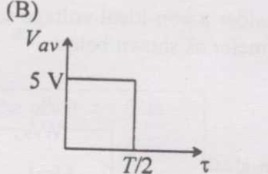
\includegraphics[width=0.3\textwidth]{17.jpg} 
      \caption{}
    \label{fig:fig17} 
\end{figure}
\item \begin{figure}[H]
      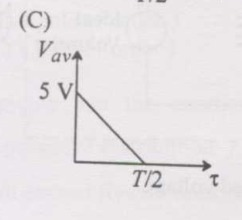
\includegraphics[width=0.3\textwidth]{18.jpg} 
      \caption{}
    \label{fig:fig18} 
\end{figure}
\item  \begin{figure}[H]
      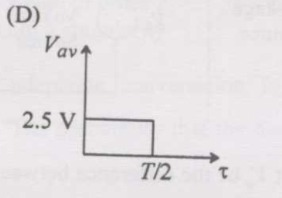
\includegraphics[width=0.3\textwidth]{19.jpg} 
      \caption{}
    \label{fig:fig19} 
\end{figure}
\end{enumerate}

\hfill(GATE IN 2007)
\item In the circuit shown in the following figure, the current through the $1\ \Omega$ resistor is
\begin{figure}[H]
    \centering
      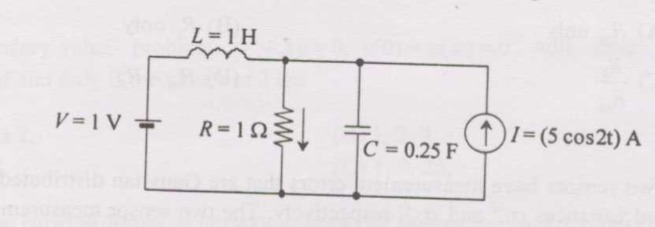
\includegraphics[width=0.6\textwidth]{20.jpg} 
      \caption{}
    \label{fig:fig20} 
\end{figure}
\begin{multicols}{2}
\begin{enumerate}
\item $(1+5\cos 2t)\ \mathrm{A}$  
\item $(5+\cos 2t)\ \mathrm{A}$  
\item $(1-5\cos 2t)\ \mathrm{A}$  
\item $6\ \mathrm{A}$  
\end{enumerate}
\end{multicols}
\hfill(GATE IN 2007)
\item In the circuit shown in the following figure, the switch is kept closed for a long time and then opened at $t=0$.  
\begin{figure}[H]
    \centering
      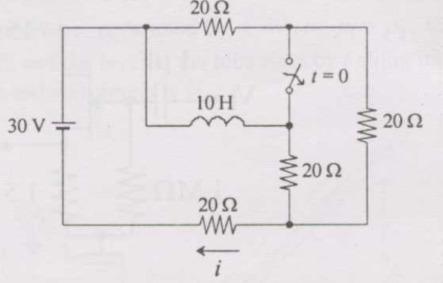
\includegraphics[width=0.6\textwidth]{21.jpg} 
      \caption{}
    \label{fig:fig21} 
\end{figure}
The values of the current $i$ just before opening the switch $(t=0^-)$ and just after opening the switch $(t=0^+)$ are, respectively
\begin{multicols}{4}
\begin{enumerate}
\item $\tfrac{3}{4}\ \mathrm{A}$ and $1\ \mathrm{A}$  
\item $\tfrac{3}{4}\ \mathrm{A}$ and $\tfrac{5}{4}\ \mathrm{A}$  
\item $1\ \mathrm{A}$ and $\tfrac{7}{6}\ \mathrm{A}$  
\item $1\ \mathrm{A}$ and $1\ \mathrm{A}$  
\end{enumerate}
\end{multicols}
\hfill(GATE IN 2007)
\item Consider the coupled circuit shown below.
\begin{figure}[H]
    \centering
      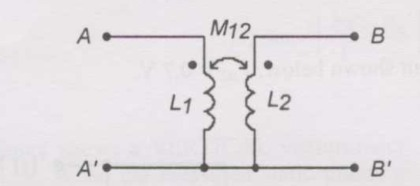
\includegraphics[width=0.6\textwidth]{22.jpg} 
      \caption{}
    \label{fig:fig22} 
\end{figure}
At angular frequency $\omega$, this circuit can be represented by the equivalent T-network.  
\begin{figure}[H]
    \centering
      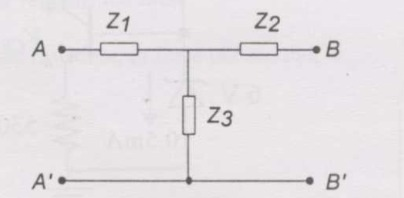
\includegraphics[width=0.6\textwidth]{23.jpg} 
      \caption{}
    \label{fig:fig23} 
\end{figure}
Indicate the correct set of expressions for the impedances of the T-network.

\begin{multicols}{2}
\begin{enumerate}
\item $Z_1 = j\omega(L_1 - M_{12}),\ Z_2 = j\omega(L_2 - M_{12}),\ Z_3 = j\omega M_{12}$  
\item $Z_1 = j\omega(L_1+M_{12}),\ Z_2 = j\omega(L_2+M_{12}),\ Z_3 = -j\omega M_{12}$  
\item $Z_1 = j\omega L_1,\ Z_2 = j\omega L_2,\ Z_3 = j\omega M_{12}$  
\item $Z_1 = j\omega(L_1+L_2+M_{12}),\ Z_2 = j\omega L_2,\ Z_3 = j\omega L_1$  
\end{enumerate}
\end{multicols}
\hfill(GATE IN 2007)
\item A FET source follower is shown in the figure below. 
\begin{figure}[H]
    \centering
      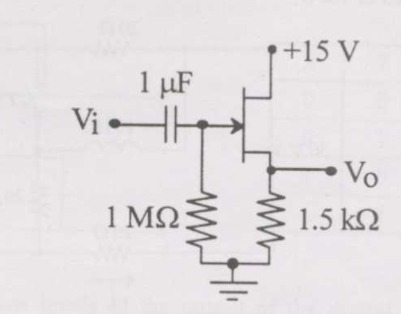
\includegraphics[width=0.6\textwidth]{24.jpg} 
      \caption{}
    \label{fig:fig24} 
\end{figure}
The nature of feedback in this circuit is  

\begin{enumerate}
\item positive current  
\item negative current  
\item positive voltage  
\item negative voltage  
\end{enumerate}
\hfill(GATE IN 2007)
\item In the circuit shown below, $V_{\mathrm{BE}} = 0.7\ \mathrm{V}$.
\begin{figure}[H]
    \centering
      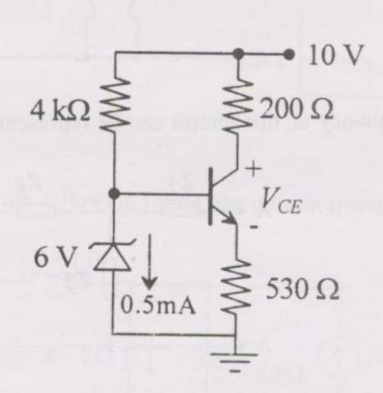
\includegraphics[width=0.6\textwidth]{25.jpg} 
      \caption{}
    \label{fig:fig25} 
\end{figure}
The $\beta$ of the transistor and $V_{CE}$ are, respectively

\begin{multicols}{4}
\begin{enumerate}
\item $19$ and $2.8\ \mathrm{V}$  
\item $19$ and $4.7\ \mathrm{V}$  
\item $38$ and $2.8\ \mathrm{V}$  
\item $38$ and $4.7\ \mathrm{V}$  
\end{enumerate}
\end{multicols}
\hfill(GATE IN 2007)
\item A well of cross-sectional area $ a_w $ is connected to an inclined tube of cross-sectional area $ a_t $ to form a differential pressure gauge as shown in the figure. When $ p_1 = p_2 $, the common liquid level is denoted by $ A $. When $ p_1 > p_2 $, the liquid level in the well is depressed to $ B $, and the level in the tube rises by $ l $ along its length such that the difference in the tube and well levels is $ h_d $.
\begin{figure}[H]
    \centering
      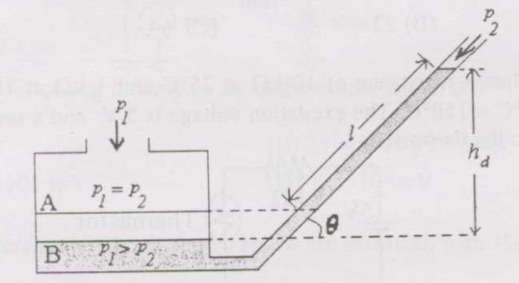
\includegraphics[width=0.6\textwidth]{26.jpg} 
      \caption{}
    \label{fig:fig26} 
\end{figure}
The angle of inclination $ \theta $ of the tube with the horizontal is:

\begin{multicols}{2}
\begin{enumerate}
\item $ \sin^{-1} \left( \dfrac{l}{h_d} - \dfrac{a_w}{a_t} \right) $
\item $ \sin^{-1} \left( \dfrac{h_d}{l} + \dfrac{a_t}{a_w} \right) $
\item $ \sin^{-1} \left( \dfrac{h_d}{l} - \dfrac{a_t}{a_w} \right) $
\item $ \sin^{-1} \left( \dfrac{h_d}{l} - \dfrac{a_w}{a_t} \right) $
\end{enumerate}
\end{multicols}
\hfill(GATE IN 2007)
\item A vertical venturimeter is shown. When the measured static pressure difference between inlet and throat$p_1 - p_2 = 30\ \mathrm{kPa}$, the flow rate was $50$ liters/s.Assume that the coefficientof dischareremains the same.
If $p_1 - p_2 = 20\ \mathrm{kPa}$, the flow rate is  
\begin{figure}[H]
    \centering
      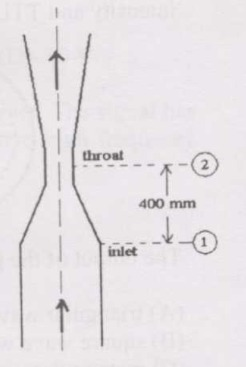
\includegraphics[width=0.6\textwidth]{27.jpg} 
      \caption{}
\label{fig:fig27} 
\end{figure}
\begin{multicols}{4}
\begin{enumerate}
\item $33.3$  
\item $39.3$  
\item $40.8$  
\item $54.2$  
\end{enumerate}
\end{multicols}
\hfill(GATE IN 2007)
\item A thermometer with time constant $\tau$ is used to measure the temperature of a liquid. If $\theta(t)$ and $\theta_i(t)$ are the excess temperatures of the thermometer and liquid, then $\lim_{t\to \infty} (\dot{\theta}(t) - \dot{\theta}_i(t))$ is  

\begin{multicols}{4}
\begin{enumerate}
\item $0$  
\item $-k$  
\item $-k\theta$  
\item $-k\tau$  
\end{enumerate}
\end{multicols}
\hfill(GATE IN 2007)
\item In a laminar flow experiment, two fluids $A$ and $B$ are pumped through straight tubes with same flow rates and pressure drops. The ratio of the dynamic viscosities $\mu_A / \mu_B$ is  

\begin{multicols}{4}
\begin{enumerate}
\item $16$  
\item $32$  
\item $64$  
\item $128$  
\end{enumerate}
\end{multicols}
\hfill(GATE IN 2007)
\item A thermistor has resistance $10\ \mathrm{k}\Omega$ at $25^\circ C$ and $1\ \mathrm{k}\Omega$ at $100^\circ C$. The range of operation is $0^\circ C - 150^\circ C$. The excitation voltage is $5\ \mathrm{V}$ and a series resistor of $1\ \mathrm{k}\Omega$ is connected to the thermistor.
\begin{figure}[H]
    \centering
      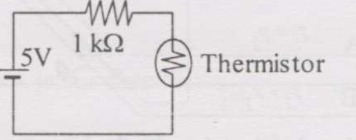
\includegraphics[width=0.6\textwidth]{28.jpg} 
      \caption{}
    \label{fig:fig28} 
\end{figure}
The power dissipated in the thermistor at $150^\circ C$ is  

\begin{multicols}{4}
\begin{enumerate}
\item $4.0\ \mathrm{mW}$  
\item $4.7\ \mathrm{mW}$  
\item $5.4\ \mathrm{mW}$  
\item $6.1\ \mathrm{mW}$  
\end{enumerate}
\end{multicols}

\hfill(GATE IN 2007)


\item A measurement system for the rotational speed of a motor is shown in the figure below. The system consists of an opaque disk attached to the motor shaft with a hole. A light source and a photodetector are placed on two sides of the disk so that whenever the hole crosses the light path, the photodetector receives light through the hole. The photodetector circuit is also shown below. Assume sufficient light intensity and TTL logic levels for the inverter.
\begin{figure}[H]
    \centering
      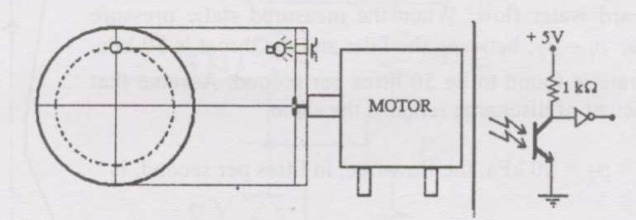
\includegraphics[width=0.6\textwidth]{29.jpg} 
      \caption{}
    \label{fig:fig29} 
\end{figure}
The output of the photodetector is a 
\begin{enumerate}
    \item triangular wave
    \item square wave with 50\% duty cycle
    \item rectangular wave with duty cycle close to unity
    \item rectangular wave with duty cycle close to zero
\end{enumerate}
\hfill(GATE IN 2007)

\item A pH electrode, being used at 25$^\circ$C, has a source resistance of $10^{10}\,\Omega$. The electrode obeys the Nernst equation perfectly. The electronic voltmeter, with which the potential is being measured, has an input impedance of $10^{12}\,\Omega$ and a gain of 100. If the pH of the analyte changes from 6.5 to 7.8, the change in voltage observed on the voltmeter is:

\begin{multicols}{2}
\begin{enumerate}
    \item less than 6.8 V
    \item between 6.8 V and 7.19 V
    \item between 7.2 V and 7.49 V
    \item greater than 7.49 V
\end{enumerate}
\end{multicols}

\hfill(GATE IN 2007)

\item The figure shows a single op-amp differential amplifier circuit.
\begin{figure}[H]
    \centering
      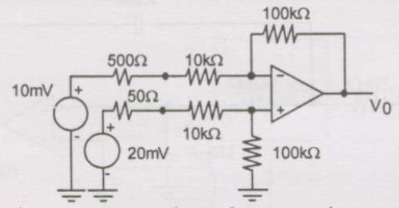
\includegraphics[width=0.6\textwidth]{30.jpg} 
      \caption{}
    \label{fig:fig30} 
\end{figure}
Which one of the following statements about the output is correct?

\begin{multicols}{2}
\begin{enumerate}
    \item $V_o \leq 95$ mV
    \item $95 < V_o \leq 98$ mV
    \item $98 < V_o \leq 101$ mV
    \item $V_o > 101$ mV
\end{enumerate}
\end{multicols}
\hfill(GATE IN 2007)
\item The three transistors in the circuit shown below are identical, with $V_{BE} = 0.7$ V and $\beta = 100$. 
\begin{figure}[H]
    \centering
      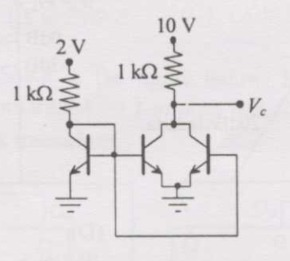
\includegraphics[width=0.6\textwidth]{31.jpg} 
      \caption{}
    \label{fig:fig31} 
\end{figure}
The voltage $V_C$ is:

\begin{multicols}{4}
\begin{enumerate}
    \item 0.2 V
    \item 2 V
    \item 7.4 V
    \item 10 V
\end{enumerate}
\end{multicols}
\hfill(GATE IN 2007)
\item The input signal shown in the figure below is fed to a Schmitt trigger. The signal has a square wave amplitude of 6 V p-p. It is corrupted by an additive high frequency noise of amplitude 8 V p-p.
\begin{figure}[H]
    \centering
      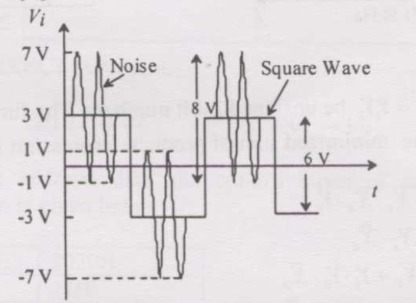
\includegraphics[width=0.6\textwidth]{32.jpg} 
      \caption{}
    \label{fig:fig32} 
\end{figure}
Which one of the following is an appropriate choice for the upper and lower trip points of the Schmitt trigger to recover a square wave of the same frequency from the corrupted input signal $V_i$?

\begin{multicols}{4}
\begin{enumerate}
    \item $\pm 8.0$ V
    \item $\pm 2.0$ V
    \item $\pm 0.5$ V
    \item 0 V
\end{enumerate}
\end{multicols}
\hfill(GATE IN 2007)
\item Consider the circuit shown below.
\begin{figure}[H]
    \centering
      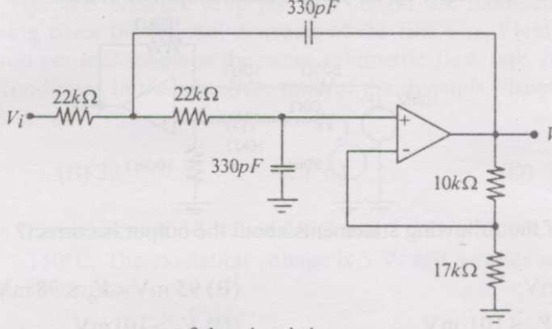
\includegraphics[width=0.6\textwidth]{33.jpg} 
      \caption{}
    \label{fig:fig33} 
\end{figure}
The correct frequency response of the circuit is:

\begin{multicols}{2}
\begin{enumerate}
    \item \begin{figure}[H]
      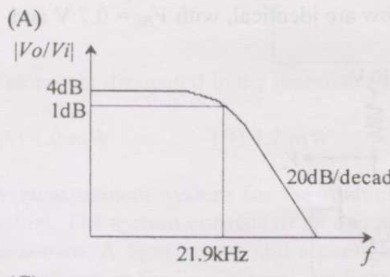
\includegraphics[width=0.3\textwidth]{34.jpg} 
      \caption{}
    \label{fig:fig34} 
\end{figure}
    \item \begin{figure}[H]
    \centering
      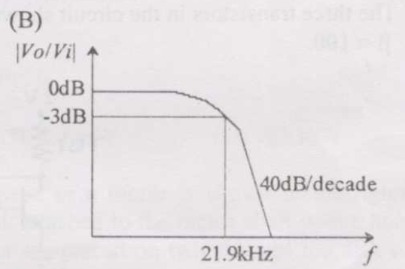
\includegraphics[width=0.3\textwidth]{35.jpg} 
      \caption{}
    \label{fig:fig35} 
\end{figure}
    \item\begin{figure}[H]
    \centering
      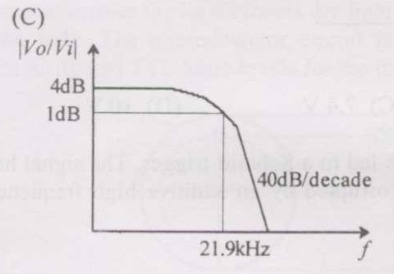
\includegraphics[width=0.3\textwidth]{36.jpg} 
      \caption{}
    \label{fig:fig36} 
\end{figure}
    \item \begin{figure}[H]
    \centering
      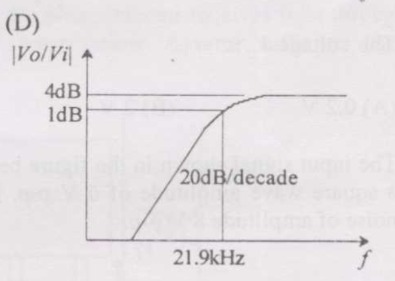
\includegraphics[width=0.3\textwidth]{37.jpg} 
      \caption{}
    \label{fig:fig37} 
\end{figure}
\end{enumerate}
\end{multicols}
\hfill(GATE IN 2007)
\item Let $ X = X_1 X_0 $ and $ Y = Y_1 Y_0 $ be unsigned 2-bit numbers. The function $ F = 1 $ if $ X > Y $ and  $F = 0 $otherwise. The minimized sum of products expression for $F$ is:


\begin{enumerate}
  \item $ Y_1 \cdot \overline{Y_0} + X_0 \cdot Y_0 + \overline{X_1} \cdot X_0 \cdot \overline{Y_1} $
  \item $ X_0\cdot  \overline{Y_1} + Y_1 \cdot \overline{Y_0} + X_1 \cdot \overline{X_0} $
  \item $ Y_1 \cdot  \overline{X_1} + Y_0 \cdot \overline{X_1} \cdot \overline{X_0} + Y_1 \cdot  Y_0 \cdot  \overline{X_0} $
  \item $ X_1 \cdot \overline{Y_1} + X_0 \cdot \overline{Y_1} \cdot \overline{Y_0} + X_1 \cdot X_0 \cdot \overline{Y_0} $
\end{enumerate}


\hfill(GATE IN 2007)

  \item A MUX circuit shown in the figure below implements a logic function $ F_1 $.
\begin{figure}[H]
    \centering
      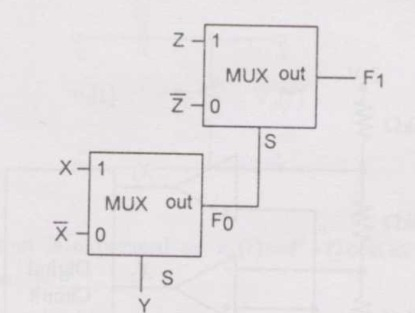
\includegraphics[width=0.6\textwidth]{38.jpg} 
      \caption{}
    \label{fig:fig38} 
\end{figure}
  The correct expression for $ F_1 $ is:

\begin{multicols}{4}
    \begin{enumerate}
      \item $ (\overline{X \oplus Y}) \oplus Z $
      \item $ \overline{\overline{(X \oplus Y)} \oplus Z} $
      \item $ (X \oplus Y) \oplus \overline{Z} $
      \item $ (X \oplus Y) + Z $
    \end{enumerate}
\end{multicols}
\hfill(GATE IN 2007)
\item A sequential circuit is shown in the figure below. Let the state of the circuit be encoded as $Q_AQ_B$. The notation $X \rightarrow Y$ implies that state $Y$ is reachable from state $X$ in a finite number of clock transitions.
\begin{figure}[H]
    \centering
      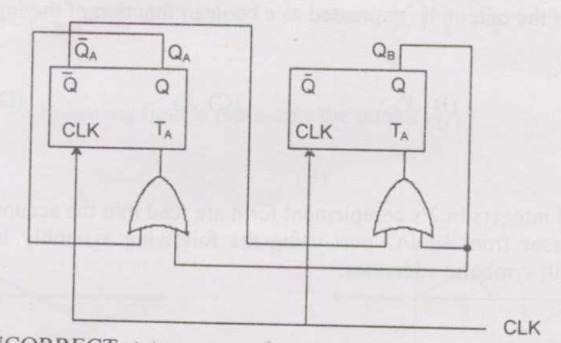
\includegraphics[width=0.6\textwidth]{39.jpg} 
      \caption{}
    \label{fig:fig39} 
\end{figure}
Identify the incorrect statement:

\begin{multicols}{4}
\begin{enumerate}
    \item $01 \rightarrow 00$
    \item $11 \rightarrow 01$
    \item $01 \rightarrow 11$
    \item $01 \rightarrow 10$
\end{enumerate}
\end{multicols}
\hfill(GATE IN 2007)
\item A snapshot of the address, data and control buses of an 8085 microprocessor executing a program is given below:
\begin{table}[H]
\begin{tabular}{|c|c|}
    \hline
    Address & 2020H \\ \hline
    Data & 24H \\ \hline
     IO/M & Logic High \\ \hline
     RD & Logic High \\ \hline
     WR & Logic Low \\ \hline
\end{tabular}
\caption{}
\label{tab:table 1}
\end{table}

The assembly language instruction being executed is:

\begin{multicols}{4}
\begin{enumerate}
    \item IN 24H
    \item IN 20H
    \item OUT 24H
    \item OUT 20H
\end{enumerate}
\end{multicols}
\hfill(GATE IN 2007)
\item The circuit shown in the figure below works as a 2-bit analog to digital converter for $0 \leq V_{in} \leq 3$ V.
\begin{figure}[H]
    \centering
      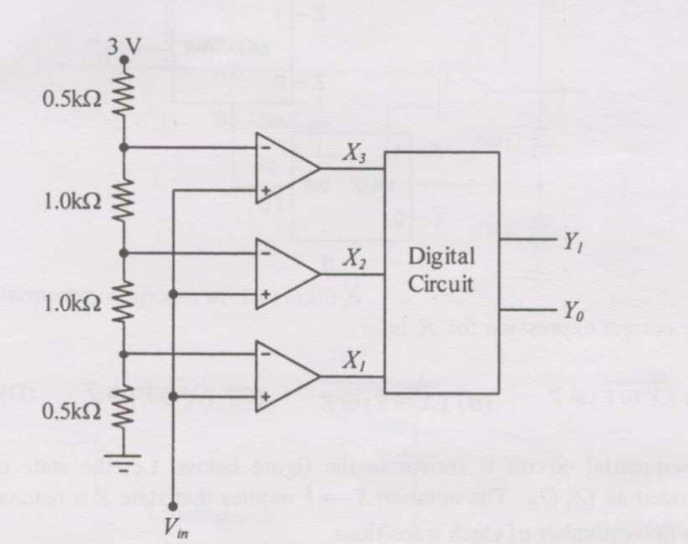
\includegraphics[width=0.6\textwidth]{40.jpg} 
      \caption{}
    \label{fig:fig40} 
\end{figure}
The MSB of the output $Y_1$, expressed as a Boolean function of the inputs $X_1$, $X_2$, $X_3$, is:

\begin{multicols}{4}
\begin{enumerate}
    \item $X_1$
    \item $X_2$
    \item $X_3$
    \item $X_1 + X_2$
\end{enumerate}
\end{multicols}
\hfill(GATE IN 2007)
\item 8-bit signed integers in 2's complement form are read into the accumulator of an 8085 microprocessor from an I/O port using the following assembly language program segment:
 \begin{verbatim}
BEGIN: IN PORT
       RAL
       JNC BEGIN
       RAR
END:   HLT
\end{verbatim}



\begin{enumerate}
    \item halts upon reading a negative number
    \item halts upon reading a positive number
    \item halts upon reading a zero
    \item never halts
\end{enumerate}

\hfill(GATE IN 2007)
\item In the circuit shown in the figure, the input signal is $v_i(t) = 5 + 3 \cos(\omega t)$. 
\begin{figure}[H]
    \centering
      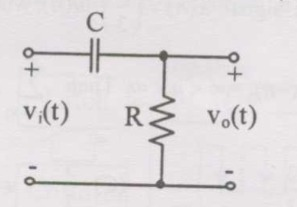
\includegraphics[width=0.6\textwidth]{41.jpg} 
      \caption{}
    \label{fig:fig41} 
\end{figure}
The steady-state output is expressed as $v_o(t) = P + Q \cos(\omega t - \phi)$. If $\omega CR = 2$, the values of $P$ and $Q$ are:

\begin{multicols}{2}
\begin{enumerate}
    \item $P = 0$, $Q = \frac{6}{\sqrt5}$
    \item $P = 0$, $Q = \frac{3}{\sqrt5}$
    \item $P = 5$, $Q = \frac{6}{\sqrt5}$
    \item $P = 5$, $Q = 3$
\end{enumerate}
\end{multicols}
\hfill(GATE IN 2007)
\item The signals $x(t)$ and $h(t)$ shown in the figures are convolved to yield $y(t)$. 
\begin{figure}[H]
    \centering
      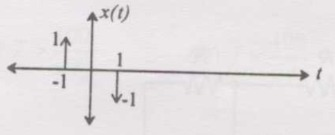
\includegraphics[width=0.6\textwidth]{42.jpg} 
      \caption{}
    \label{fig:fig42} 
\end{figure}
\begin{figure}[H]
    \centering
      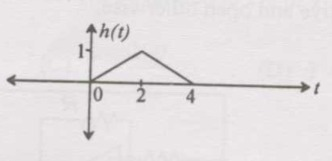
\includegraphics[width=0.6\textwidth]{43.jpg} 
      \caption{}
    \label{fig:fig43} 
\end{figure}
Which one of the following figures represents the output $y(t)$?

\begin{multicols}{2}
\begin{enumerate}
    \item \begin{figure}[H]
    \centering
      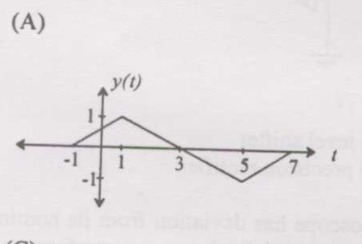
\includegraphics[width=0.3\textwidth]{44.jpg} 
      \caption{}
    \label{fig:fig44} 
\end{figure}
    \item \begin{figure}[H]
    \centering
      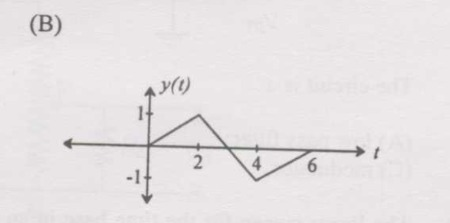
\includegraphics[width=0.3\textwidth]{45.jpg} 
      \caption{}
    \label{fig:fig45} 
\end{figure}
    \item \begin{figure}[H]
    \centering
      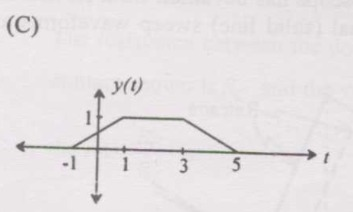
\includegraphics[width=0.3\textwidth]{46.jpg} 
      \caption{}
    \label{fig:fig46} 
\end{figure}
    \item \begin{figure}[H]
    \centering
      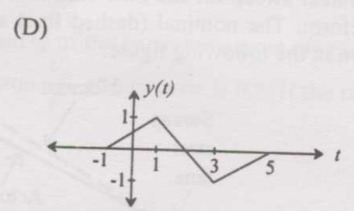
\includegraphics[width=0.3\textwidth]{47.jpg} 
      \caption{}
 \label{fig:fig47} 
\end{figure}
\end{enumerate}
\end{multicols}
\hfill(GATE IN 2007)
\item Consider the discrete-time signal $x(n) = (-1)^n u(n)$, where $u(n) = 1$ for $n \geq 0$, and define $y(n) = x(-n)$. Then $\sum_{n=-\infty}^{\infty} y(n)$ equals:

\begin{multicols}{4}
\begin{enumerate}
    \item $-2/3$
    \item $2/3$
    \item $3/2$
    \item $3$
\end{enumerate}
\end{multicols}
\hfill(GATE IN 2007)
\item Let the signal $x(t)$ have the Fourier transform $X(\omega)$. Consider the signal $y(t) = x(t - t_a)$ where $t_a$ is an arbitrary delay. The magnitude of the Fourier transform of $y(t)$ is:

\begin{multicols}{4}
\begin{enumerate}
    \item $|X(\omega) \cdot [\omega]|$
    \item $|X(\omega)| \cdot \omega$
    \item $\omega^2 \cdot |X(\omega)|$
    \item $|(\omega)||X(\omega) \cdot e^{-j\omega t_a}|$
\end{enumerate}
\end{multicols}
\hfill(GATE IN 2007)
\item In the circuit shown below, the switch (S) is closed whenever the input voltage ($V_{in}$) is positive and open otherwise.
\begin{figure}[H]
    \centering
      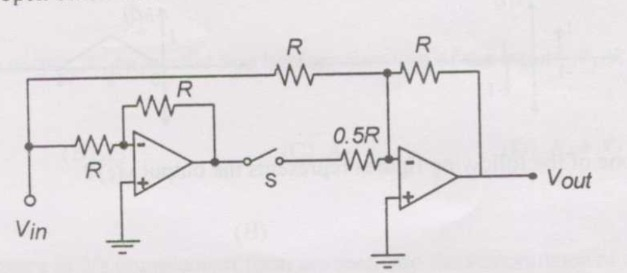
\includegraphics[width=0.6\textwidth]{48.jpg} 
      \caption{}
\label{fig:fig48} 
\end{figure}
The circuit is a:

\begin{multicols}{2}
\begin{enumerate}
    \item low pass filter
    \item level shifter
    \item modulator
    \item precision rectifier
\end{enumerate}
\end{multicols}
\hfill(GATE IN 2007)
\item The linear sweep for the time base in an oscilloscope has deviation from its nominal waveform. The nominal (dashed line) and actual (solid line) sweep waveforms are shown. 
\begin{figure}[H]
    \centering
      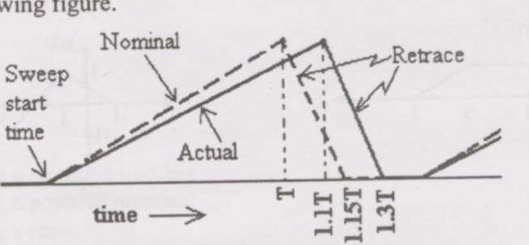
\includegraphics[width=0.6\textwidth]{49.jpg} 
      \caption{}
    \label{fig:fig49} 
\end{figure}
A 5 V p-p sine wave with a frequency of 1 kHz will be measured on the oscilloscope as a sine wave with:

\begin{multicols}{2}
\begin{enumerate}
    \item 4.45 V p-p and 1 kHz frequency
    \item 5 V p-p and 1 kHz frequency
    \item 5 V p-p and 1.1 kHz frequency
    \item 5 V p-p and 1.15 kHz frequency
\end{enumerate}
\end{multicols}
\hfill(GATE IN 2007)
\item The pulse width $T$ of an asynchronous pulse is measured by a counter with an edge-triggered clock of known frequency $f_c$.
\begin{figure}[H]
    \centering
      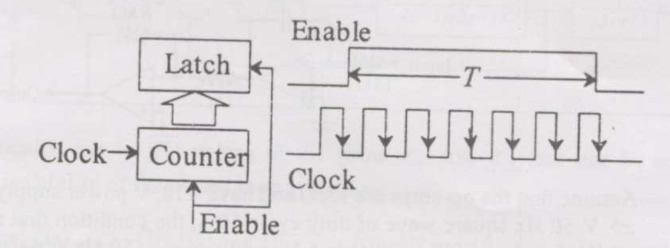
\includegraphics[width=0.6\textwidth]{50.jpg} 
      \caption{}
    \label{fig:fig50} 
\end{figure}
The counter counts while Enable is high and is reset otherwise. The counter output is latched by the negative edge of Enable. The measured pulse width is taken to be $N$ times the clock period. Assuming no overflow, the measurement error will be limited to $x\%$ of $T$ if:

\begin{multicols}{4}
\begin{enumerate}
    \item $T > \dfrac{100}{xf_c}$
    \item $T < \dfrac{100}{xf_c}$
    \item $T > \dfrac{200}{xf_c}$
    \item $T < \dfrac{200}{xf_c}$
\end{enumerate}
\end{multicols}
\hfill(GATE IN 2007)
\item A potentiometer of total resistance $R_T$ with a sliding contact is shown. 
\begin{figure}[H]
    \centering
      \includegraphics[width=0.6\textwidth]{51.jpg} 
      \caption{}
    \label{fig:fig51} 
\end{figure}
The resistance between points P and Q is $R_C$ and the voltage ratio $V$ at this point is 0.5. If $\dfrac{R_L}{R_T} = 1$, then the ratio $\dfrac{R_C}{R_T}$ is:

\begin{multicols}{4}
\begin{enumerate}
    \item $\dfrac{-1 + \sqrt{5}}{2}$
    \item $\dfrac{1 + \sqrt{5}}{2}$
    \item $-1 + \sqrt{5}$
    \item $1 + \sqrt{5}$
\end{enumerate}
\end{multicols}
\hfill(GATE IN 2007)
\item Consider the triangular wave generator shown.
\begin{figure}[H]
    \centering
      \includegraphics[width=0.6\textwidth]{52.jpg} 
      \caption{}
    \label{fig:fig52} 
\end{figure}
Assume ideal op-amps and $\pm2$ V supply. If the input is a +5 V, 50 Hz square wave with 50\% duty cycle, the condition that results in a triangular wave of 5 V peak-to-peak and 50 Hz frequency at the output is:

\begin{multicols}{4}
\begin{enumerate}
    \item $RC = 1$
    \item $R/C = 1$
    \item $R/C = 5$
    \item $C/R = 5$
\end{enumerate}
\end{multicols}
\hfill(GATE IN 2007)

\item Two signals of peak-to-peak voltages 5 V and 2 V are fed to Channel 1 and Channel 2 of an oscilloscope. Vertical sensitivity is 1 V/div. The sine waves have identical frequency and phase. Trigger is manual at +1.25 V on Channel 1. 

Which trace correctly depicts Channel 2?
\begin{figure}[H]
	\centering
      \includegraphics[width=0.6\textwidth]{53.jpg} 
      \caption{}
    \label{fig:fig53} 
\end{figure}
\begin{enumerate}
    \item      \begin{figure}[H]
      \includegraphics[width=0.15\textwidth]{54.jpg} 
      \caption{}
    \label{fig:fig54} 
\end{figure} P
    \item \begin{figure}[H]
      \includegraphics[width=0.15\textwidth]{55.jpg} 
      \caption{}
    \label{fig:fig55} 
\end{figure}  Q
    \item           \begin{figure}[H]
      \includegraphics[width=0.15\textwidth]{56.jpg} 
      \caption{}
    \label{fig:fig56} 
\end{figure} R
    \item  \begin{figure}[H]
      \includegraphics[width=0.15\textwidth]{57.jpg} 
      \caption{}
    \label{fig:fig57} 
\end{figure}   S
\end{enumerate}
\hfill(GATE IN 2007)

\item A chamber is heated with a heater of max power 1000 W. The steady-state power-temperature slope is 2 W/°C. Heater power is the sum of a proportional controller output (band = 200\%) and a constant offset of 500 W. The temperature achieved for a set point of 300°C is:

\begin{multicols}{4}
\begin{enumerate}
    \item 260°C
    \item 60°C
    \item 275°C
    \item 150°C
\end{enumerate}
\end{multicols}
\hfill(GATE IN 2007)

\item A cascade control system with proportional controllers is shown.
\begin{figure}[H]
    \centering
      \includegraphics[width=0.6\textwidth]{58.jpg} 
      \caption{}
	\label{fig:fig58} 
\end{figure}
Theoretically, the largest values of gains $K_1$ and $K_2$ that can be set without causing instability of the closed loop system are:

\begin{multicols}{4}
\begin{enumerate}
    \item 10 and 100
    \item 100 and 10
    \item 10 and 10
    \item $\infty$ and $\infty$
\end{enumerate}
\end{multicols}
\hfill(GATE IN 2007)

\item The ECG of a patient is recorded using three standard frontal plane leads. If the cardiac vector is oriented at 45° to Lead I and has a magnitude of 3 mV, the voltages seen on Leads I, II, and III are:

\begin{multicols}{2}
\begin{enumerate}
    \item 1.50, 2.27, and 0.77 mV
    \item 2.12, 0.77, and 2.89 mV
    \item 2.12, 3.15, and 1.03 mV
    \item 2.12, 2.89, and 0.77 mV
\end{enumerate}
\end{multicols}
\hfill(GATE IN 2007)

\item Light of intensity $I_0$ is equally divided and passed through two cuvettes $P_1$ and $P_2$ containing analyte at concentrations $c$ and $0.5c$, respectively. Path lengths are 4 cm and 1 cm; cross-sectional areas are 1 cm² and 3 cm². The ratio of absorbances in $P_1$ and $P_2$ is:

\begin{multicols}{4}
\begin{enumerate}
    \item 1.5
    \item $\dfrac{8}{3}$
    \item 3
    \item 8
\end{enumerate}
\end{multicols}
\hfill(GATE IN 2007)

\item The H-D curves of two X-ray films $F_1$ and $F_2$ are shown. 
\begin{figure}[H]
    \centering
      \includegraphics[width=0.6\textwidth]{59.jpg} 
      \caption{}
    \label{fig:fig59} 
\end{figure}
For the same change in exposure, $F_1$ has:


\begin{enumerate}
    \item higher contrast than $F_2$ but same fog level
    \item lower contrast than $F_2$ but same fog level
    \item higher contrast and higher fog level than $F_2$
    \item lower contrast than $F_2$ but higher fog level
\end{enumerate}
\hfill(GATE IN 2007)

\begin{center}
\textbf{Common Data Question}
\end{center}

\textbf{Common Data for Questions 71, 72, 73:}

Consider the op-amp circuit shown in the figure below.
\begin{figure}[H]
    \centering
      \includegraphics[width=0.6\textwidth]{60.jpg} 
      \caption{}
    \label{fig:fig60} 
\end{figure}
  \item If $ V_1 = 0.2\,V $, $ V_2 = 0.6\,V $, and $ V_o = -0.7\,V $, and the op-amp is ideal, the value of $ R_1 $ is:

  \begin{multicols}{4}
  \begin{enumerate}
    \item 5 k$\Omega$
    \item 10 k$\Omega$
    \item 15 k$\Omega$
    \item 20 k$\Omega$
  \end{enumerate}
  \end{multicols}
\hfill(GATE IN 2007)

  \item Let $ V_1 = V_2 = V_c \sin 2\pi f t $ and $ R_1 = 20\,k\Omega $. The op-amp has a slew rate of 0.5 V/$\mu$s with its other parameters being ideal. The values of $ V_c $ and $ f $ for which the amplifier output will have no distortion are, respectively:

  \begin{multicols}{2}
\begin{enumerate}
    \item 0.1 V and 300 kHz
    \item0.5 V and 300 kHz
    \item 0.1 V and 30 kHz
    \item 0.5 V and 30 kHz
  \end{enumerate}
  \end{multicols}
\hfill(GATE IN 2007)

  \item Let $ V_1 = V_2 = 0 $ and $ R_1 = 20\,k\Omega $. Assume that the op-amp is ideal except for a non-zero input bias current. What is the value of $ R_2 $ for the output voltage of the op-amp to be zero?

  \begin{multicols}{4}
	  \begin{enumerate}
    \item 2.2 k$\Omega$
    \item 9.1 k$\Omega$
    \item 20 k$\Omega$
    \item 100 k$\Omega$
  \end{enumerate}
  \end{multicols}
\hfill(GATE IN 2007)

\textbf{Common data for Questions 74 and 75:}  
The following figure represents a proportional control scheme of a first order system with transportation lag.  
\begin{figure}[H]
    \centering
      \includegraphics[width=0.6\textwidth]{61.jpg} 
      \caption{}
    \label{fig:fig61} 
\end{figure}
\item 
The angular frequency in rad/s at which the loop phase lag becomes 180$^\circ$ is  

\begin{multicols}{4}
\begin{enumerate}
\item 0.408  
\item 0.818  
\item 1.56  
\item 2.03  
\end{enumerate}
\end{multicols}
\hfill(GATE IN 2007)

\item 
The steady state error for a unit step input when the gain $K_c = 1$ is  

\begin{multicols}{4}
\begin{enumerate}
\item 1/4  
\item 1/2  
\item 1  
\item 2  
\end{enumerate}
\end{multicols}
\hfill(GATE IN 2007)

\begin{center}
    \textbf{Linked Answer Questions}
\end{center}
\textbf{Statement for Linked Answer Questions 76 \& 77:}  
Blood flow through a straight segment of an artery is measured using a Doppler flowmeter. The probe is oriented at an angle of 45$^\circ$ to the longitudinal axis of the artery. It is known that Doppler shift is proportional to the velocity of blood in the direction of propagation of sound from the probe and the frequency generated from the probe. The velocity of sound in blood is 1500 m/s and the maximum blood flow velocity to be measured is 110 cm/s.  

\item 
Signal processing limitations constrain the maximum Doppler shift to be less than 3 kHz. The maximum source frequency (probe output), to the nearest MHz, should be  

\begin{multicols}{4}
\begin{enumerate}
\item 2 MHz  
\item 3 MHz  
\item 5 MHz  
\item 10 MHz  
\end{enumerate}
\end{multicols}
\hfill(GATE IN 2007)

\item 
In Q.76, if the piezoelectric crystal of the probe is made of quartz (Young's modulus $Y=8\times10^{10}\,\text{N/m}^2$, $\rho = 2.65\times10^3\,\text{kg/m}^3$), the minimum thickness of the crystal required to resonate at the frequency determined above, to the nearest mm, is  

\begin{multicols}{4}
\begin{enumerate}
\item 1 mm  
\item 2 mm  
\item 3 mm  
\item 4 mm  
\end{enumerate}
\end{multicols}
\hfill(GATE IN 2007)

\textbf{Statement for Linked Answer Questions 78 \& 79:}  
Consider the circuit shown in the following figure.
\begin{figure}[H]
    \centering
      \includegraphics[width=0.6\textwidth]{62.jpg} 
      \caption{}
    \label{fig:fig62} 
\end{figure}
\item 
The correct input-output relationship between $Y$ and $(X_1,X_2)$ is  

\begin{multicols}{4}
\begin{enumerate}
\item $Y = X_1 + X_2$  
\item $Y = X_1 X_2$  
\item $Y = X_1 \bar{X_2}$  
\item $Y = \bar{X_1} \bar{X_2}$  
\end{enumerate}
\end{multicols}
\hfill(GATE IN 2007)

\item 
The D flip-flops are initialized to $Q_2 Q_1 Q_0 = 000$. After 1 clock cycle, $Q_2 Q_1 Q_0$ is equal to  

\begin{multicols}{4}
\begin{enumerate}
\item 011  
\item 010  
\item 100  
\item 101  
\end{enumerate}
\end{multicols}
\hfill(GATE IN 2007)

\textbf{Statement for Linked Answer Questions 80 \& 81:}  

The numerical aperture of a step index fiber in air (refractive index = 1) is 0.39. The diameter of the core is 200 $\mu$m.
\item The angle of acceptance when the fiber is used in water (refractive index = 1.33) is closest to  

\begin{multicols}{4}
\begin{enumerate}
\item 15$^\circ$  
\item 16$^\circ$  
\item 17$^\circ$  
\item 18$^\circ$  
\end{enumerate}
\end{multicols}
\hfill(GATE IN 2007)

\item 
Two experiments are conducted in which light is launched into the fiber from a uniformly distributed planar source kept 5 mm away from the tip. In the first experiment ($E_1$), both the source and the fiber are in air. In the second experiment ($E_2$), both the source and the fiber are in water. Neglecting absorption and reflection between the source and the tip, the ratio of the amount of light coupled into the fiber in $E_2$ to the amount of light coupled into the fiber in $E_1$ is closest to  

\begin{multicols}{4}
\begin{enumerate}
\item 0.5  
\item 1.0  
\item 1.4  
\item 1.9  
\end{enumerate}
\end{multicols}
\hfill(GATE IN 2007)

\textbf{Statement for Linked Answer Questions 82 \& 83:}  

A push-pull capacitive displacement transducer is interfaced to a differential amplifier and an ADC as shown in the figure below.  
\begin{figure}[H]
    \centering
      \includegraphics[width=0.6\textwidth]{63.jpg} 
      \caption{}
    \label{fig:fig63} 
\end{figure}
Note that the bridge supply and the analog reference input for the ADC are derived from the same 10 V DC source. 

\item The change in capacitance for full scale displacement is 5\% for the capacitors. The gain of the differential amplifier for utilization of the full range of the ADC (which is $\pm 10$ V) is
\begin{multicols}{4}
\begin{enumerate}
\item 10  
\item 20  
\item 30 
\item 40  
\end{enumerate}
\end{multicols}
\hfill(GATE IN 2007)

\item If the supply voltage to the bridge decreases by 5\%, the sensitivity of the measurement system
\begin{multicols}{2}
\begin{enumerate}
\item decreases by 5\%  
\item does not change  
\item increases by 5\%  
\item increases by 200\%  
\end{enumerate}
\end{multicols}
\hfill(GATE IN 2007)

\textbf{Statement for Linked Answer Questions 84 \& 85:}  

A transfer function with unity DC gain has three poles at -1, -2, and -3 and no finite zeros. A plant with this transfer function is connected with a proportional controller of gain $K$ in the forward path, in a unity feedback configuration.  

\item The transfer function is
\begin{multicols}{2}
\begin{enumerate}
\item $\dfrac{s}{(s-1)(s-2)(s-3)}$
\item $\dfrac{6}{(s+1)(s+2)(s+3)}$
\item $\dfrac{s}{(s+1)(s+2)(s+3)}$
\item $\dfrac{6}{(s-1)(s-2)(s-3)}$
\end{enumerate}
\end{multicols}
\hfill(GATE IN 2007)

\item If the root locus plot of the closed loop system passes through the points $\pm j\sqrt{11}$, the maximum value of $K$ for stability of the unity feedback closed loop system is
\begin{multicols}{4}
\begin{enumerate}
\item $\sqrt{11}$  
\item 6  
\item 10  
\item $\dfrac{6}{\sqrt{11}}$  
\end{enumerate}
\end{multicols}
\hfill(GATE IN 2007)

\end{enumerate}
\end{document}


